% future/QC.tex (7ab78678da33efd03a237070761df1ca888bee48)

\section{Quantum Computing}
\label{sec:future:Quantum Computing}

양자 컴퓨팅 (QC) 에 대한 아이디어는 수십년 전으로 거슬러
갑니다만~\cite{RichardPFeynman1959RoomAtBottom,Bennett:1973:LRC:1664562.1664568,RichardFeynman1986QuantumMechanicalComputers},
양자 컴퓨터를 구축하기 위한 기술은 최근 들어서야
나타났습니다~\cite{KamranKarimi2011D-WaveAdiabatic,IBM2016QuantumExperience}.
그러나 전통적 기술에 대한 언론에 비해서조차도 대단한 일은 만들지
못했습니다~\cite{Economist2017QuantumComputingTechnologyQuarterly}.
이 섹션은 IBM 의 Quantum Experience 웹사이트~\cite{IBM2016QuantumExperience} 과
외부의 문헌에 대한 리뷰에 기반해서 이 기술의 상태에 대한 간략한 개괄을
제공합니다.
이 개괄은 비록 QC 가 애타는 가능성을 약속하긴 하지만, 급격하게 개선되고 있는
고전적 컴퓨팅 기술과 발견들 등을 포함해서 극복해야 하는 많은 문제들이 존재함을
이야기합니다.

이 섹션은 2017년 초의 관점에서의 양자 컴퓨팅에 대한 개괄을 제공합니다.
이는 양자 계산에만 집중함을 알아두시기 바랍니다.
양자 통신과 양자 암호화는 훨씬 진보되었으며, 실제로 쓰이고 있으며, 이 섹션의
범위 밖입니다.
\iffalse

The ideas behind quantum computing (QC) go back
decades~\cite{RichardPFeynman1959RoomAtBottom,Bennett:1973:LRC:1664562.1664568,RichardFeynman1986QuantumMechanicalComputers},
but the technology to construct quantum computers has appeared
only recently~\cite{KamranKarimi2011D-WaveAdiabatic,IBM2016QuantumExperience}.
It has nevertheless generated considerable excitement,
even outside of the traditional technical
press~\cite{Economist2017QuantumComputingTechnologyQuarterly}.
This section gives a brief overview of the state of this
technology, based on use of IBM's Quantum Experience
website~\cite{IBM2016QuantumExperience} and on a superficial
literature review.
This overview indicates that although QC promises some
tantalizing possibilities, there are significant challenges
that it must overcome, including rapidly improving classic-computing
techniques and heuristics.

This section gives an overview of quantum computing from the perspective
of early 2017.
Note that this is concerned only with quantum computation.
Quantum communication and quantum cryptography are far more
advanced, are used in practice, and are beyond the scope of
this section.
\fi

Section~\ref{sec:future:Quantum Computing Players}
은 QC 시스템들에 대한 작업을 하고 있는 더 뛰어난 회사들에 대한 개괄을
제공합니다.
Section~\ref{sec:future:Quantum Computing Progress}
은 오늘날의 QC 하드웨어 트렌드들의 짧은 평가를 보입니다.
Section~\ref{sec:future:Quantum Computing Challenges}
은 QC 가 실제로 널리 쓰이기 위해서는 극복해야 하는 몇가지 도전사항들을
분석합니다.
Section~\ref{sec:future:Outlook} 은 QC 가 ``세계를 집어삼키기'' 위해 어떤 일이
있어야 할지 예측해 봅니다.
마지막으로,
Section~\ref{sec:future:QC Summary and Conclusions}
에서는 요약과 몇가지 결론을 냅니다.
\iffalse

Section~\ref{sec:future:Quantum Computing Players}
gives an overview of some of the more prominent companies working
with QC systems.
Section~\ref{sec:future:Quantum Computing Progress}
presents a brief evaluation of QC hardware trends to date.
Section~\ref{sec:future:Quantum Computing Challenges}
analyzes several challenges that QC must surmount in order to achieve
widespread use in practice.
Section~\ref{sec:future:Outlook} speculates on what must happen for QC
to ``take over the world''.
Finally,
Section~\ref{sec:future:QC Summary and Conclusions}
presents a summary and a few conclusions.
\fi

\subsection{Quantum Computing Players}
\label{sec:future:Quantum Computing Players}

이 섹션은 QC 방면의 상업적 선수들 일부에 대한 개괄을 제공합니다.

D-Wave Systems~\cite{D-WaveSystemsHomePage} 는 d-wave
superconductor~\cite{MHSAmin2000D-Wave-superconductor} 에 기반한 양자 컴퓨팅
시스템을 2011년에 공개했습니다~\cite{WikipediaD-WaveSystems}.
이 시스템은 굉장히 이야기되고
연구되었습니다~\cite{KamranKarimi2011D-WaveAdiabatic}.
D-Wave 가 정말로 양자 특성을 보여주는지에 대해선 많은 질문이
있었습니다만~\cite{SeungWooShin2014IsDwaveQuantum}, 최근의 조짐은 양자 효과가
정말로 존재한다는 것입니다~\cite{PhysRevA.91.042314,PhysRevX.4.021041}.
D-Wave 에게는 여러 고객들과 협력사들이
있습니다~\cite{JeffreyBurt2014Google-QC-Chip,PatrickHarris2015QC-Google-NASA-DWave,ToddRWeiss2013Google-QC-AI-Lab}.
또한, D-Wave 는 2017년에 존재하는 2,048-qubit 을 가진, 많은 수의 quantum bits
또는 \emph{qubits}~\cite{WikipediaD-WaveSystems} 의 상업적 기계를 가진, 이
영역에서의 패배한 적 없는
챔피언입니다~\cite{AgamShah2016D-Wave-2000-qubit,BradJones2017D-Wave2000Sale}..
그렇다고는 하나, 이 시스템들은 범용적 qubit 들을 갖추지는 못했고 최적화 문제에
특화된 qubit 들만을 갖췄습니다.
\iffalse

This section provides an overview of several of the commercial
players in the QC arena.

D-Wave Systems~\cite{D-WaveSystemsHomePage}
released a quantum computing system
in 2011~\cite{WikipediaD-WaveSystems}, based on a d-wave
superconductor~\cite{MHSAmin2000D-Wave-superconductor}.
This system has been heavily discussed and
studied~\cite{KamranKarimi2011D-WaveAdiabatic}.
There has been some question as to whether D-Wave really exhibits quantum
properties~\cite{SeungWooShin2014IsDwaveQuantum}, but more recent
indications are that quantum effects really are
present~\cite{PhysRevA.91.042314,PhysRevX.4.021041}.
D-Wave has a number of customers and
collaborators~\cite{JeffreyBurt2014Google-QC-Chip,PatrickHarris2015QC-Google-NASA-DWave,ToddRWeiss2013Google-QC-AI-Lab}.
In addition, D-Wave is the undisputed champion in the area of commercially
available machines with large numbers of quantum bits, or
\emph{qubits}~\cite{WikipediaD-WaveSystems},
with a 2,048-qubit system delivered in
2017~\cite{AgamShah2016D-Wave-2000-qubit,BradJones2017D-Wave2000Sale}.
That said, these systems do not feature general-purpose qubits, but
rather qubits that are specialized to optimization problems.
\fi

D-Wave 와의 협업에 더해서, Google 은 UCSB 와 QC
메모리~\cite{JaikumarVijayan2015Google-UCSB-QC-Memory} 를 포함해서 QC
하드웨어에 대해 작업을 해왔습니다.

Intel 은 Google, NASA, 그리고 USRA 와의 제휴 하에 \$50M 를
투자했습니다~\cite{StaceyHigginbotham2015Intel-QC-invest-50M}.

Microsoft 와 UCSB 는 2004 년부터 QC 에 대해 협업을
해왔고~\cite{PedroHernandez2014MicrosoftStationQ-QC} Microsoft 는 최근에 새로운
Quantum 사단~\cite{PedroHernandez2016Microsoft-QC} 를 형성했습니다.
일부는 Microsoft 가 QC programming language 의 리더가 될거라 여깁니다.
Microsoft 는 quatum chemistry 가 QC 의 킬러 애플리케이션이 될거라
믿습니다~\cite{TomSimonite2017QC-MS-Chemistry}.
\iffalse

In addition to its collaboration with D-Wave, Google has been working
with UCSB on QC hardware, including
QC memory~\cite{JaikumarVijayan2015Google-UCSB-QC-Memory}.

Intel is investing \$50M in quantum computing in partnership
with Google, NASA, and USRA~\cite{StaceyHigginbotham2015Intel-QC-invest-50M}.

Microsoft and UCSB have been collaborating on QC since
2004~\cite{PedroHernandez2014MicrosoftStationQ-QC}
and Microsoft has recently formed a new Quantum
division~\cite{PedroHernandez2016Microsoft-QC}.
Some regard Microsoft to be the leader in QC programming languages.
Microsoft believes that quantum chemistry will be the killer app
for QC~\cite{TomSimonite2017QC-MS-Chemistry}.
\fi

IBM 은 1973 년의 QC computation 의 열역학 가역성에 대한 Bennett 의
작업~\cite{Bennett:1973:LRC:1664562.1664568} 과 1980 년의 Josephson
기술~\cite{1980:1663086} 에 집중한 IBM Journal of Research and Development 를
포함해서 오랜기간의 양자에 대한 작업 기록을 갖고 있습니다.
IBM 은 scanning tunneling microscopy~\cite{Binnig1982SurfaceSTM} 과 Don Eigler
에 의해 원자 단위에서 ``IBM'' 을 쓰기 위해
사용된~\cite{MalcolmWBrowne1990AFM-IBM} atomic force
microscope~\cite{1986PhRvL..56..930B} 와 함께 이 기본 작업을 계속하고
있습니다~\cite{Binnig1982SurfaceSTM}.
\iffalse

IBM has a long record of quantum work, including Bennett's
1973 work on the thermodynamic reversibility of QC
computation~\cite{Bennett:1973:LRC:1664562.1664568} and a 1980 issue
of IBM Journal of Research and Development focusing on Josephson
technology~\cite{1980:1663086}.
IBM continued this groundbreaking work with scanning tunneling
microscopy~\cite{Binnig1982SurfaceSTM}
and the atomic force microscope~\cite{1986PhRvL..56..930B},
which was famously used by Don Eigler to spell ``IBM'' on the atomic
scale~\cite{MalcolmWBrowne1990AFM-IBM}.
\fi

더 최근에 IBM 은 D-Wave 의 것보다 적은 qubit 을 갖지만 D-Wave 와 달리 범용
qubit 에 집중한 quantum-computing 하드웨어에
집중했습니다~\cite{BradJones2017IBM-QC-Announce,RobertHackett2017IBM-QC-Announce,AgamShah2017IBM-QC-50-qubit,DarioGill2017IBM-Universal-QC}.
이에 더해서, IBM 은 Yel Universal 의 transmon~\cite{WikipediaTransMon}
작업~\cite{PhysRevA.76.042319} 에 기반한 자신의 QC
하드웨어~\cite{IBM2016QuantumExperience,ArsTechnica2016IBMQuantumExperience,MikeVizard2017IBM-QC-Cloud}
를 공개적으로 사용 가능하게 내놓은 첫 사례입니다.
이 작업은 일관성 시간을 수십 마이크로세컨드로 증가시키도록
확장되었습니다~\cite{PhysRevLett.107.240501,PhysRevLett.111.080502,PhysRevB.86.100506}.
IBM 의 공개적으로 사용가능한 QC 하드웨어는 제한된 얽힘을 갖는 다섯개의 qubit
만을 제공함에도 불구하고 첫해에만 40,000 명의 서로 다른 사용자들에 의해 275,000
개의 실험들을 수행했습니다.
2017 년 5월에 이르러, 16개, 17개 qubit 시스템들이 IBM 에서 사용 가능합니다.

짧게 말해서, QC 는 상당한 짜릿함을 만들어내고 있고 상당한 투자를 받고 있습니다.
아직 알려지지 않은 QC 선수가 주요한 game-changing breakthrough 를 이끌 가능성도
상당히 있습니다.
그 사이에, 다음 섹션은 QC 영역에서의 기술적 진행 내용을 알아봅니다.
\iffalse

More recently, IBM has been focusing on quantum-computing hardware with
fewer qubits than that of D-Wave, but unlike D-Wave focuses on
general-purpose
qubits~\cite{BradJones2017IBM-QC-Announce,RobertHackett2017IBM-QC-Announce,AgamShah2017IBM-QC-50-qubit,DarioGill2017IBM-Universal-QC}.
In addition, IBM is the first to allow public access to its QC
hardware~\cite{IBM2016QuantumExperience,ArsTechnica2016IBMQuantumExperience,MikeVizard2017IBM-QC-Cloud},
which is based on transmon~\cite{WikipediaTransMon} work at
Yale University~\cite{PhysRevA.76.042319}.
This work has been extended
to increase coherence times into the tens of
microseconds~\cite{PhysRevLett.107.240501,PhysRevLett.111.080502,PhysRevB.86.100506}.
IBM's publicly available QC hardware was used by about 40,000 different
users running 275,000 experiments within its first
year~\cite{SeanMichaelKerner2017IBM-QC-API},
despite offering only five qubits having constrained entanglement.
As of May 2017, sixteen- and seventeen-qubit systems are available
from IBM.

In short, QC is generating great excitement and receiving substantial
investment.
It is quite possible that a yet-as-unknown QC player will drive a
major game-changing breakthrough.
In the meantime, the next section evaluates technical progress in the
QC arena.
\fi

\subsection{Quantum Computing Progress}
\label{sec:future:Quantum Computing Progress}

QC 시스템들은 여러 기술적 분야에서 Moore 의 법칙과 같은 스타일의 상당한 진보를
만들어 왔습니다.
\iffalse

QC systems have been making substantial Moore's-Law-style progress
in a number of technical areas.
\fi

\begin{table}
\centering\footnotesize
\begin{tabular}{l|r|r|r}
	&	&	& Years per \\
System
	& Availability
		& Qubits
			& Doubling \\
\hline
\hline
D-Wave One
	& May 2011
		& 128
			& 1.4 \\
\hline
D-Wave Two
	& May 2013
		& 512
			& 1.9 \\
\hline
D-Wave 2X
	& Aug 2015
		& 1152
			& 1.7 \\
\hline
D-Wave 2000Q
	& Jan 2017
		& 2048
			& --- \\
\end{tabular}
\caption{D-Wave Qubit Growth Rate}
\label{tab:future:D-Wave Qubit Growth Rate}
\end{table}

예를 들어서, Table~\ref{tab:future:D-Wave Qubit Growth Rate} 은 D-Wave 의
시스템들, 발매된 날짜, qubit 의 갯수, 그리고 그 해로부터 현재까지 qubit 갯수를
두배로 늘리는데 걸린 시간을 보입니다.
이 데이터는 극단적으로 제한된 데이터이긴 하지만 qubit 에 있어서의 Moore 의 법칙
같은 성장세를 보입니다.
뒤따르는 논의에서는 (낙관적인) 긴 시점에서의 qubit 양을 두배로 늘리는데 걸리는
1.4 년의 시간을 사용할 겁니다.
하지만 IBM Quantum Experience 의 2016 년 5월에 제공한 내용은 5개의 qubit 만을
갖습니다만, 2017년 5월에 내놓은 것은 16개의 qubit 을 갖습니다.
이는 qubit 을 두배로 만드는데 걸리는 시간은 8 \emph{달} 이 안걸림을
의미합니다만, IBN 이 이 추세를 유지할지는 계속해서 지켜보아야 할겁니다.
한편으로는, 만약 QC 가 고전적 컴퓨팅에 의해 만들어진 기술을 잘 사용할 수
있다면, qubit 의 갯수가 갑자기 수십수백배로 들어날 가능성도 있습니다.

또다른 방법은 물론 주어진 문제를 해결하는데에 필요한 qubit 의 갯수를 줄이는
것일 겁니다~\cite{SergeyBravyi2017-QC-SimulateFermionicHamiltonians}.
하지만, Section~\ref{sec:future:Error Rate} 에서 보게 되겠지만, quantum error
correction 의 필요는 필요한 qubit 의 갯수를 늘립니다.
\iffalse

For example, Table~\ref{tab:future:D-Wave Qubit Growth Rate} shows D-Wave's systems,
availability dates, numbers of qubits, and years per doubling
from that year to the present.
This data hints at a Moore's-Law-like growth in qubits, albeit from
an extremely limited data set.
Further discussion will use the (optimistic) long-term qubit
doubling duration of 1.4 years.
IBM Quantum Experience's May 2016 offering had but five qubits, but its
May 2017 offering has sixteen qubits.
This represents a qubit doubling duration of less than eight \emph{months},
but it remains to be seen whether IBM can sustain this pace.
% bc -l: 12*l(2)/l(16/5)
On the other hand, if QC can make good use of the process technology
developed for classic computing, there is some possibility that the number
of qubits might increase quite suddenly by many orders of magnitude.

Another approach is of course to reduce number of qubits required for a
given problem~\cite{SergeyBravyi2017-QC-SimulateFermionicHamiltonians}.
However, as will be seen in Section~\ref{sec:future:Error Rate}, the need for
quantum error correction increases the number of qubits required.
\fi

\begin{figure}[tb]
\centering
\resizebox{3in}{!}{\rotatebox{270}{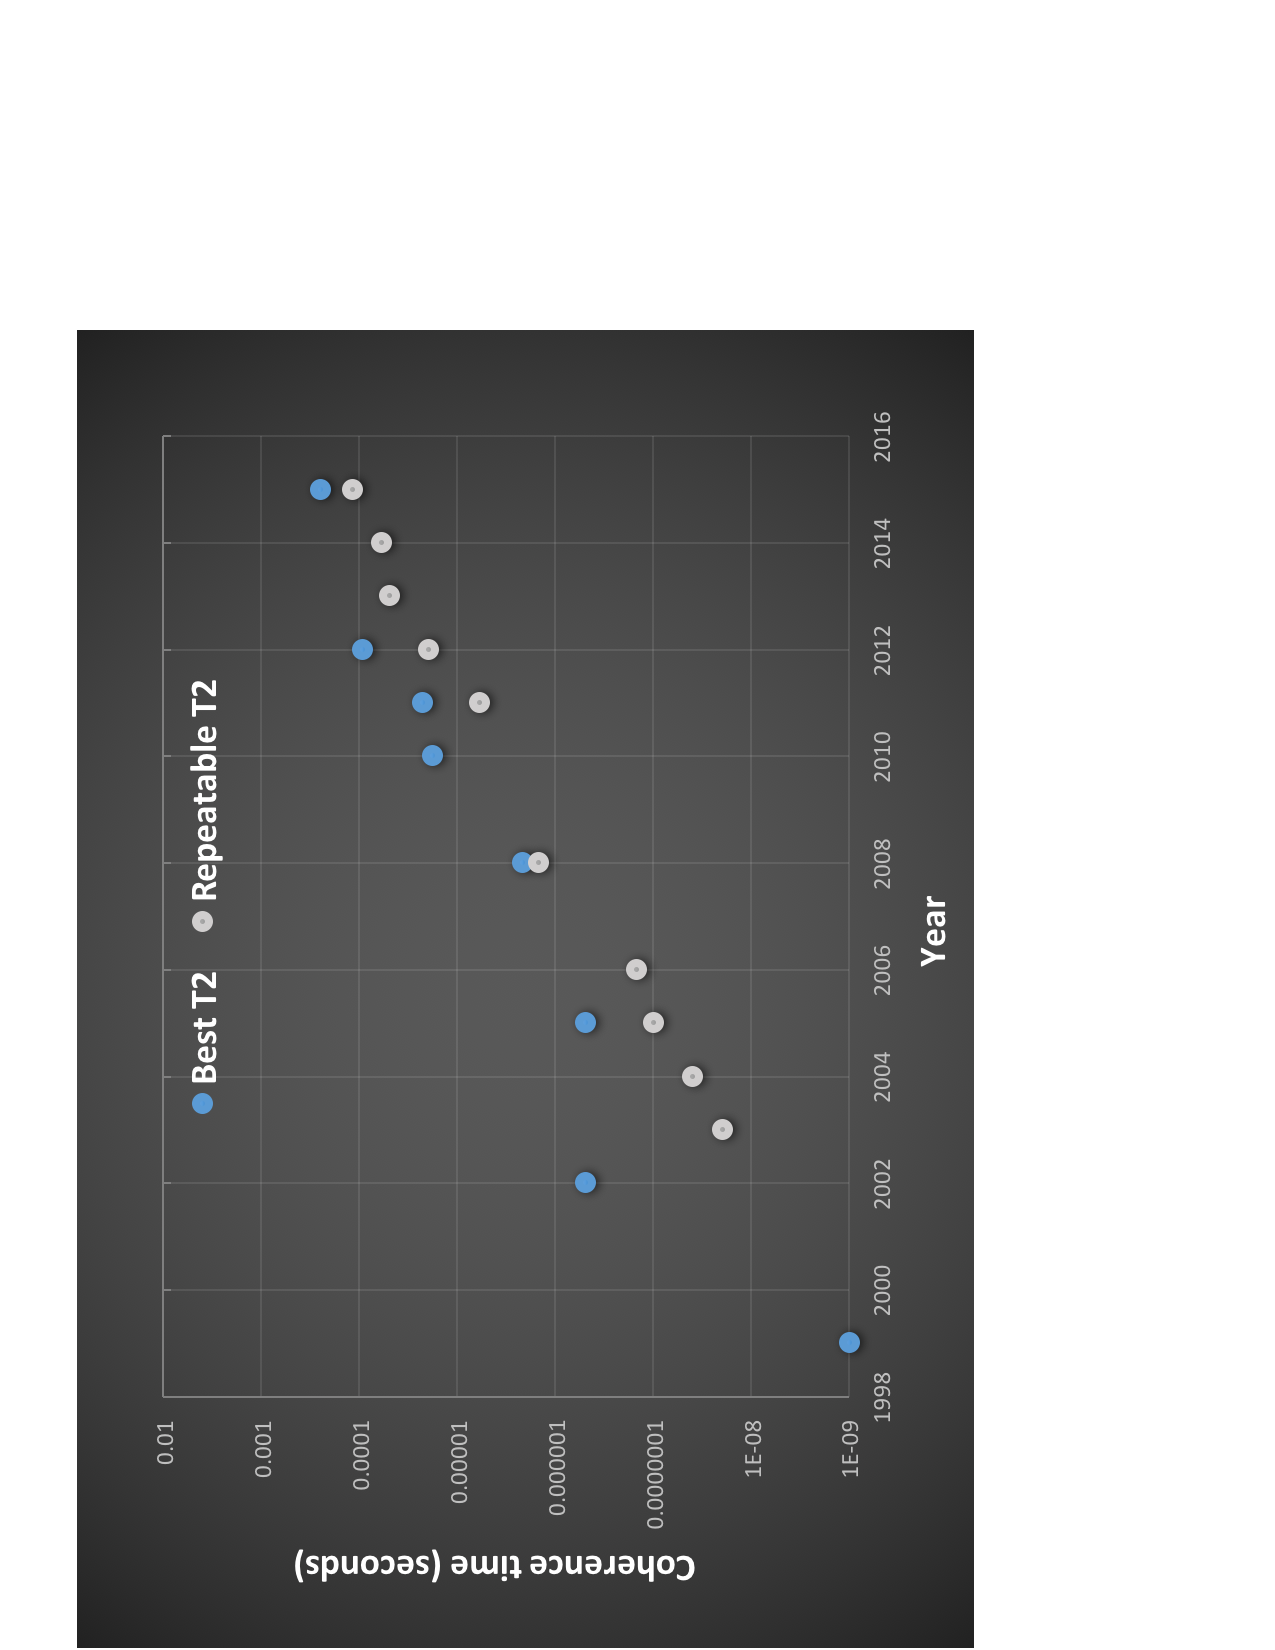
\includegraphics{future/T2h1lc19xmqrdlsor}}}
\caption{Coherence Time Trend}
\label{fig:future:Coherence Time Trend}
\end{figure}

QC 의 발전에 있어서의 또다른 핵심 요소는 decoherence time 입니다.
QC decoherence 는 qubit 들이 불안정하며 시간의 흐름에 따라 붕괴하게 된다는
사실에서 기인합니다.
물론, 이는 전례없는 것은 아닙니다: 무엇보다도, classical computing 의 어디에나
존재하는 dynamic RAM 은 주기적으로 재충전 되어야만 합니다.
하지만, 누군가가 qubit 들을 재충전 할 수 있는 실용적인 방법을 내놓기
전까지는~\cite{GiorgioColangelo2017QC-SpinAngleAmplitude},
decoherence time 을 늘리는 것이 quantum 알고리즘이 더 많은 처리를 할 수 있도록
해줄 겁니다.
Superconducting qubit 을 위한 coherence time 은
Figure~\ref{fig:future:Coherence Time Trend}~\cite{IBM2016QuantumExperience}
에 보인 것처럼 매년 두배가 될겁니다.
이 트렌드를 외삽해 보면 10년 내로 10초의 coherence time 이 가능해 질 것으로, 더
복잡하고 긴시간 동작하는 QC 알고리즘들이 실용적 영역으로 들어올 수 있게 할
것이고 또한 복잡한 error-correction 방법들의 필요를 줄일 것이라 예쌍할 수
있습니다.
\iffalse

Another key element of QC progress is decoherence time.
QC decoherence results from the fact that qubits are fragile, and
decay over time.
Of course, this is not unprecedented: After all, classical computing's
ubiquitous dynamic RAM must be periodically refreshed.
However, until someone comes up with a practical way to refresh
qubits~\cite{GiorgioColangelo2017QC-SpinAngleAmplitude},
increasing decoherence time allows a quantum algorithm to do more
processing.
Coherence time for superconducting qubits seems to be doubling every year,
as shown in
Figure~\ref{fig:future:Coherence Time Trend}~\cite{IBM2016QuantumExperience}.
Extrapolating this trend suggests that 10-second coherence times might
be available in ten years time, which would bring more complex and
long-running QC algorithms into the realm of practicality, and might
also reduce the need for complex error-correction schemes.
\fi

마지막으로, entangle 될 수 있는 qubit 의 갯수 (그리고 entanglement 기간을)
늘리는 것은 Shor's integer-factorization
알고리즘~\cite{Shor:1997:PAP:264393.264406,Kendon:2006:ERS:2011698.2011704} 과
같은 양자 알고리즘들에 중요합니다.
Murphy 의 법칙은 entangle 될 수 있는 qubit 의 갯수를 늘리는 것은 decoherence
time 을 줄일 것이라 이야기 합니다만, 시간이 지나봐야 알 수 있을 겁니다.

Quantum-state readout 은 더 정확해 질 것이라는 애타는 힌트가
있습니다만~\cite{GiorgioColangelo2017QC-SpinAngleAmplitude}, 이런 기술들이 QC
에 적용될 것인가에 대해서는(sensing 과 분광학에서와는 대조적으로) 확실치
않습니다.
\iffalse

Finally, increasing the number of qubits that can be
entangled (and the duration of the entanglement) is important for
quantum algorithms such as Shor's integer-factorization
algorithm~\cite{Shor:1997:PAP:264393.264406,Kendon:2006:ERS:2011698.2011704}.
Murphy's Law would suggest that increasing the number of qubits that
can be entangled would also decrease decoherence time, but time will tell.

There are some tantalizing hints that quantum-state readout might become
more accurate~\cite{GiorgioColangelo2017QC-SpinAngleAmplitude},
but it is not yet clear that these techniques apply to QC
(as opposed to sensing and spectroscopy).
\fi

연구자들은 최근들어 수십 microkelvins 에서의 gaseous 상태의 3,000 개 rubidium
원자들 entangle 하는데에
성공했습니다만~\cite{RobertMcConnell2015QC-Entangle3000Atoms}, 이게 현재로써는
non-gasuous qubit 집합으로 구성되는 QC 시스템에 어떻게 적용될 수 있을지는
확실치 않습니다.
그러나, 현재의 보고서들은 entanglement 가능성의 합리적인 외삽을 가능하게 할만큼
충분한 데이터를 제공하고 있지 않습니다.\footnote{
	보고서의 문제라기보다는 아마도 편집자의 문제일 가능성이 큽니다.}
QC 에 연관된 추세는 모호해 보입니다.

이런 모든 진보들에도 불구하고, QC 는 다음 섹션의 주제이기도 한 상당한 문제에
직면해 있습니다.
\iffalse

Researchers recently achieved entanglement of 3,000
rubidium atoms in gaseous state at a few tens of
microkelvins~\cite{RobertMcConnell2015QC-Entangle3000Atoms},
though it is unclear how this could be adapted for use in
a QC system, which currently feature highly structured non-gaseous
collections of qubits.
Nevertheless, the current literature does not appear to provide enough
data to permit reasonable extrapolation of entanglement capabilities.\footnote{
	Which is quite possibly the fault of the editor rather than that
	of the literature.}
Trends regarding QC operation times seem to be similarly obscure.

Despite all this progress, QC face significant challenges, which are
the subject of the next section.
\fi

\subsection{Quantum Computing Challenges}
\label{sec:future:Quantum Computing Challenges}

QC 에서의 발전은 흥분되고 보기 좋았습니다만, 이 시스템들은 여전히 관습적
컴퓨팅의 표준에서는 상당히 조잡합니다.
IBM 의 Scott Crowder 가 말했듯, ``1940년대의
반복입니다''~\cite{BradJones2017IBM-QC-Crowder}.
비교를 위해 보자면, 가장 오래된 온전한 컴퓨터인 University of Melbourne 의
1949년도 CSIRAC~\cite{CSIRACMuseumVictoria,CSIRACUniversityMelbourne} 는 1\,KHz
의 코어 클락 주파수로 동작했고, 30\,kW 의 전력을 소모했으며, 3 metric ton 의
무게에, 2,000 개의 진공관 튜브로 구성되었고, 수은 지연선 (Acoustic Mercury
Delay Line) 으로 구현한 768 word 의 RAM 을 가졌습니다.
그리고 마지막의 두가지 요소는 왜 이게 ``운영가능한'' 게 아니라 ``온전한''
것인지에 대한 이유로, 기계적 수은도 600-volt 의 노출된 전선도 2017 년도엔
선호할 만해 보이지 않기 때문입니다.\footnote{
	둘 다 1960년대 초에는 받아들일 만 했습니다.
	2060년대의 주민들은 2017년도의 평범한 실례의 숫자들에 마찬가지로
	끔찍해할 것임에 의심의 여지가 없습니다.}
따라서 한때 CSIRAC 의 메인 메모리로 동작했던 강철관은 수은이 텅빈채이고 전선은
전류를 머금고 있지 않습니다.
더 나아가서, CSIRAC 이후로, 관들은 트랜지스터에 대체되어 구식이 되었고
트랜지스터 역시 결국은 집적회로의 여러 세대들로 인해 구식이 되었습니다.
수은 지연선은 유리 지연선으로 대체되어 구식이 되었고, 유리 지연선은 자기 코어
메모리로, 자기 코어 메모리는 반도체 DRAM 으로 대체되어왔고, DRAM 은 곧
non-volatile RAM (NVRAM) 으로 대체될 것으로 보입니다.
\iffalse


Progress on QC has been exciting and good to see, but these systems are
still quite crude by the standards of conventional computing.
As Scott Crowder of IBM put it,
``It's the 1940s again''~\cite{BradJones2017IBM-QC-Crowder}.
For purposes of comparison, the oldest intact computer, the
University of Melbourne's 1949
CSIRAC~\cite{CSIRACMuseumVictoria,CSIRACUniversityMelbourne},
ran at a core clock frequency of 1\,kHz, consumed 30\,kW of power,
weighs three metric tons,
is constructed of 2,000 vacuum tubes, and has 768 words of RAM
implemented with acoustic mercury delay lines.
And these last are two reasons why it is ``intact'' rather than
``operational'', given that
neither metallic mercury nor exposed 600-volt wiring are
looked upon favorably in 2017.\footnote{
	Both were considered to be perfectly acceptable as late as the
	early 1960s.
	Which is OK.
	The denizens of the 2060s will be no doubt be equally horrified
	by any number of unremarkable 2017 practices.}
The steel tubes that once served as CSIRAC's main memory are therefore
empty of mercury and the wiring is therefore free of current.
Furthermore, since CSIRAC, tubes have been obsoleted by discrete
transistors which were in turn obsoleted by multiple generations of
integrated circuits.
Mercury delay lines were obsoleted by glass delay lines which were
obsoleted by magnetic core memory which were obsoleted by
semiconductor DRAM, which might be on its way to being obsoleted
by non-volatile RAM (NVRAM).
\fi

그러나, CSIRAC 는 처음으로 게임을 하고 음악을 재생할 수 있는 첫번째 컴퓨터였던
것으로 알려져 있습니다.
비슷하게, 우린 미래의 QC 시스템들이 현재의 프로토타입들과는 상당히 다를 것이라
예상할 수 있지만, CSIRAC 와 마찬가지로, 현재의 QC 프로토타입들이 상당한
마일스톤을 찍을 것이라 기대해 볼 수 있습니다.

개선이 필요한 QC 분야를 더 들여다보기 위해,
Section~\ref{sec:future:Programming Model} 는 QC 프로그래밍 모델에 (그리고 일부
영역에 수수께끼를 풀려는 노력으로) 생기는 도전적 문제들을 들여다보고,
Section~\ref{sec:future:Error Rate} 에서는 qubit error rate 을 둘러싼 도전적
문제들을 보고,
Section~\ref{sec:future:Thermodynamics} 에서는 항상 불편한 열역학의 법칙에 의해
생기는 전력 효율성 문제를 이야기하며,
Section~\ref{sec:future:Heuristics} 에서는 고전적 컴퓨터들과 heuristic 의
조합과의 경쟁적 도전사항들에 대해 간략히 알아보고
Section~\ref{sec:future:Mathematical Advances} 에서는 수학자들로부터 나올 수
있는 경쟁적 도전사항들에 대한 힌트를 알아봅니다.
\iffalse

Nevertheless, the CSIRAC is believed to be the first computer to
play a game and to play music.
Similarly, we should expect future QC systems to look much different
than current prototypes, but we nevertheless have reason to hope that,
like CSIRAC, current QC prototypes will achieve notable milestones.

To shine some light on QC areas needing improvement,
Section~\ref{sec:future:Programming Model} looks at challenges posed by the QC
programming model (and attempts to demystify some aspects),
Section~\ref{sec:future:Error Rate} looks at challenges surrounding qubit
error rates,
Section~\ref{sec:future:Thermodynamics} presents energy-efficiency challenges
posed by the ever-inconvenient Laws of Thermodynamics,
Section~\ref{sec:future:Heuristics} gives an overview of competitive
challenges from the combination of classical computers and heuristics,
and
Section~\ref{sec:future:Mathematical Advances} hints at possible competitive
challenges from mathematicians.
\fi

\subsubsection{Programming Model}
\label{sec:future:Programming Model}

\begin{figure}[tb]
\centering
\resizebox{2.5in}{!}{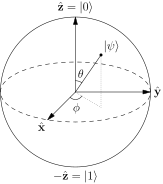
\includegraphics{future/Bloch_Sphere}}
\caption{Qubit as Bloch Sphere}
\label{fig:future:Qubit as Bloch Sphere}
\end{figure}

QC 프로그래밍 모델은 classic-computing 경험을 가진 개발자들을 위해 최대한
맞춰져 있습니다.
이 섹션의 나머지 부분에서는 qubit, quantum entanglement, 그리고 QC 하드웨어와
classic computer 하드웨어 사이의 과계에 대해 다룹니다.
\iffalse

The QC programming model is at best an acquired taste for developers
with classic-computing experience.
The remainder of this section covers qubits,
quantum entanglement,
and
the likely relationship between QC hardware and classic computer hardware.
\fi

\paragraph{Qubit}

Qubit 은 classic-computing 의 bit 과 비슷한 종류의 것인데, 단지 그런 종류일
뿐입니다.
Qubit 의 특성은:
\iffalse

A qubit is sort of like a classic-computing bit, but only sort of.
A qubit is said to:
\fi

\begin{enumerate}
\item	Figure~\ref{fig:future:Qubit as Bloch Sphere} 에 보인 것과 같이, Block
	sphere 로 나타내어집니다.
\item	측정될 때에 0 ($\ket{0}$) 또는 1 ($\ket{1}$) 로 붕괴되는데, 어느 값으로
	붕괴될지에 대한 확률은 $\ket{0}$ 과 $\ket{1}$ 로부터의 상대적 거리를
	Z-축으로 투영한 값의 함수로 계산됩니다.
	따라서, 이 Bloch sphere 의 수식에서의 qubit 은 1 또는 0 으로 측정될
	50\% 의 확률을 갖고 있으며, 45\textdegree-북쪽 위도의 qubit 은 1 로
	측정될 확률 14\% 와 0 으로 측정될 확률 86\% 를 갖습니다.
	이 상황은 기본적으로 개발자들이 sphere 보다는 실선을---또는
	classic-computing bit 을---선호하게 합니다.
\item	(측정 오퍼레이션에 더해서) Bloch sphere 위에서의 순환만을 지원합니다.
\iffalse

\item	Be represented by a Bloch sphere, as shown in
	Figure~\ref{fig:future:Qubit as Bloch Sphere}.
\item	Collapse to a zero ($\ket{0}$) or a one ($\ket{1}$) if measured,
	with probability being a function of the relative distance from
	$\ket{0}$ and $\ket{1}$, but projected onto the Z-axis.
	Thus, a qubit on the equator of the Bloch sphere has a 50\%
	probability of being measured as a one or as a zero, while
	a qubit on the 45\textdegree-north latitude would have
	a 14\% chance of being measured as one and 86\% chance
	of being measured as zero.
	This situation naturally causes developers to prefer a line
	segment---or a classic-computing bit---over a sphere.
\item	Support only rotations on the Bloch sphere (in addition to
	the measurement operation).
\fi
\end{enumerate}

Block sphere 의 필요는 주로 현재 qubit 을 나타내는, 물리적 실체들에서 현재
행해질 수 있는 quantum-mechanical 오퍼레이션ㄷ르의 제약인 \#3 에 의한 것입니다.

IBM 의 Quantum Experience 에 의해 지원되는 기본적인 non-entangling
오퍼레이터들은 다음과 같습니다:
\iffalse

It appears that the need for a Bloch sphere is mainly dictated by \#3,
the limitations on the quantum-mechanical operations currently available
on the physical entities that represent qubits.

The basic non-entangling operators supported by IBM's Quantum Experience
are as follows:
\fi

\begin{description}
\item[\qop{H}\,:]
	X-Z 축으로 Block-sphere 를 180\degree{} ($\pi$ radian), 즉 X-Z 축의
	45\degree{} 선만큼 회전시킵니다.  이는 $\ket{0}$ 를 X-축의 양의 부분이
	Bloch sphere 와 만나는 지점까지 회전시키고, $\ket{1}$ 를 X-축의 음의
	부분이 Bloch sphere 와 만나는 지점까지 회전시킵니다.
	어느 경우든, 우린 50\% 1이고 50\% 0인 qubit 을 얻게 됩니다.
	\iffalse

	Rotate 180\degree{} ($\pi$ radians) about the Bloch-sphere
	X-Z axis, that is, about the 45\degree{} line on the
	X-Z plane.  This rotates $\ket{0}$ to the point at which the
	positive X-axis intersects the Bloch sphere, and rotates $\ket{1}$
	to the point at which the negative X-axis intersects the Bloch
	sphere.
	Either way, we get a qubit that is 50\% one and 50\% zero.
	\fi
\item[\qop{S}\,:]
	Bloch-sphere 를 Z-축으로 90\degree{} ($\frac{\pi}{2}$ radian) 만큼
	회전시켜서 $\ket{0}$ 나 $\ket{1}$ 상태의 qubit 에는 아무 변화도
	일으키지 않습니다.
	\iffalse

	Rotate 90\degree{} ($\frac{\pi}{2}$ radians) about the
	Bloch-sphere Z-axis, which has no effect on qubits in the
	$\ket{0}$ or $\ket{1}$ states.
	\fi
\item[\qop{S}$^{\bm{\dagger}}$:]
	Bloch-sphere 를 Z-축으로 $-90\degree$ ($-\frac{pi}{2}$ radian) 만큼
	회전시켜서, $\ket{0}$ 나 $\ket{1}$ 상태의 qubit 에는 아무 변화도
	일으키지 않습니다.
	이 오퍼레이터는 \qop{S} 의 반대입니다.
	\iffalse

	Rotate $-90\degree$ ($-\frac{\pi}{2}$ radians) about the
	Bloch-sphere Z-axis, which has no effect on qubits in the
	$\ket{0}$ or $\ket{1}$ states.
	This operator is the inverse of \qop{S}.
	\fi
\item[\qop{T}\,:]
	Bloch-sphere 를 Z-축으로 45\degree{} ($\frac{\pi}{4}$ radian)
	회전시켜서, $\ket{0}$ 나 $\ket{1}$ 상태의 qubit 에는 아무 변화도
	일으키지 않습니다.
	\iffalse

	Rotate 45\degree{} ($\frac{\pi}{4}$ radians) about the
	Bloch-sphere Z-axis, which has no effect on qubits in the
	$\ket{0}$ or $\ket{1}$ states.
	\fi
\item[\qop{T}$^{\bm{\dagger}}$:]
	Bloch-sphere 를 Z-축으로 $-45\degree{}$ ($-\frac{\pi}{4}$ radian)
	회전시켜서, $\ket{0}$ 나 $\ket{1}$ 상태의 qubit 에는 아무 변화도
	일으키지 않습니다.
	이 오퍼레이터는 \qop{T} 의 반대입니다.
	\iffalse

	Rotate $-45\degree$ ($-\frac{\pi}{4}$ radians) about the
	Bloch-sphere Z-axis, which has no effect on qubits in the
	$\ket{0}$ or $\ket{1}$ states.
	This operator is the inverse of \qop{T}.
	\fi
\item[\qop{X}\,:]
	Bloch-sphere 를 X-축으로 180\degree{} ($\pi$ radian) 만큼 회전시켜서
	$\ket{0}$ 를 $\ket{1}$ 로, 그리고 그 반대로도 만듭니다.
	\iffalse

	Rotate 180\degree{} ($\pi$ radians) about the Bloch-sphere
	X-axis, which takes $\ket{0}$ to $\ket{1}$ and vice versa.
	\fi
\item[\qop{Y}\,:]
	Bloch-sphere 를 Y-축으로 180\degree{} ($\pi$ radian) 회전시켜서 역시
	$\ket{0}$ 를 $\ket{1}$ 로, 그리고 그 반대로도 만듭니다.
	\iffalse

	Rotate 180\degree{} ($\pi$ radians) about the Bloch-sphere
	Y-axis, which also takes $\ket{0}$ to $\ket{1}$ and vice versa.
	\fi
\item[\qop{Z}\,:]
	Bloch-sphere 를 Z-축으로 180\degree{} ($\pi$ radian) 회전시켜서
	$\ket{0}$ 나 $\ket{1}$ 상태의 qubit 에는 아무 변화도 일으키지 않습니다.
	\iffalse

	Rotate 180\degree{} ($\pi$ radians) about the Bloch-sphere
	Z-axis, which has no effect on qubits in the $\ket{0}$ or
	$\ket{1}$ states.
	\fi
\end{description}

\begin{figure}[tb]
\centering
\resizebox{2.5in}{!}{\rotatebox{270}{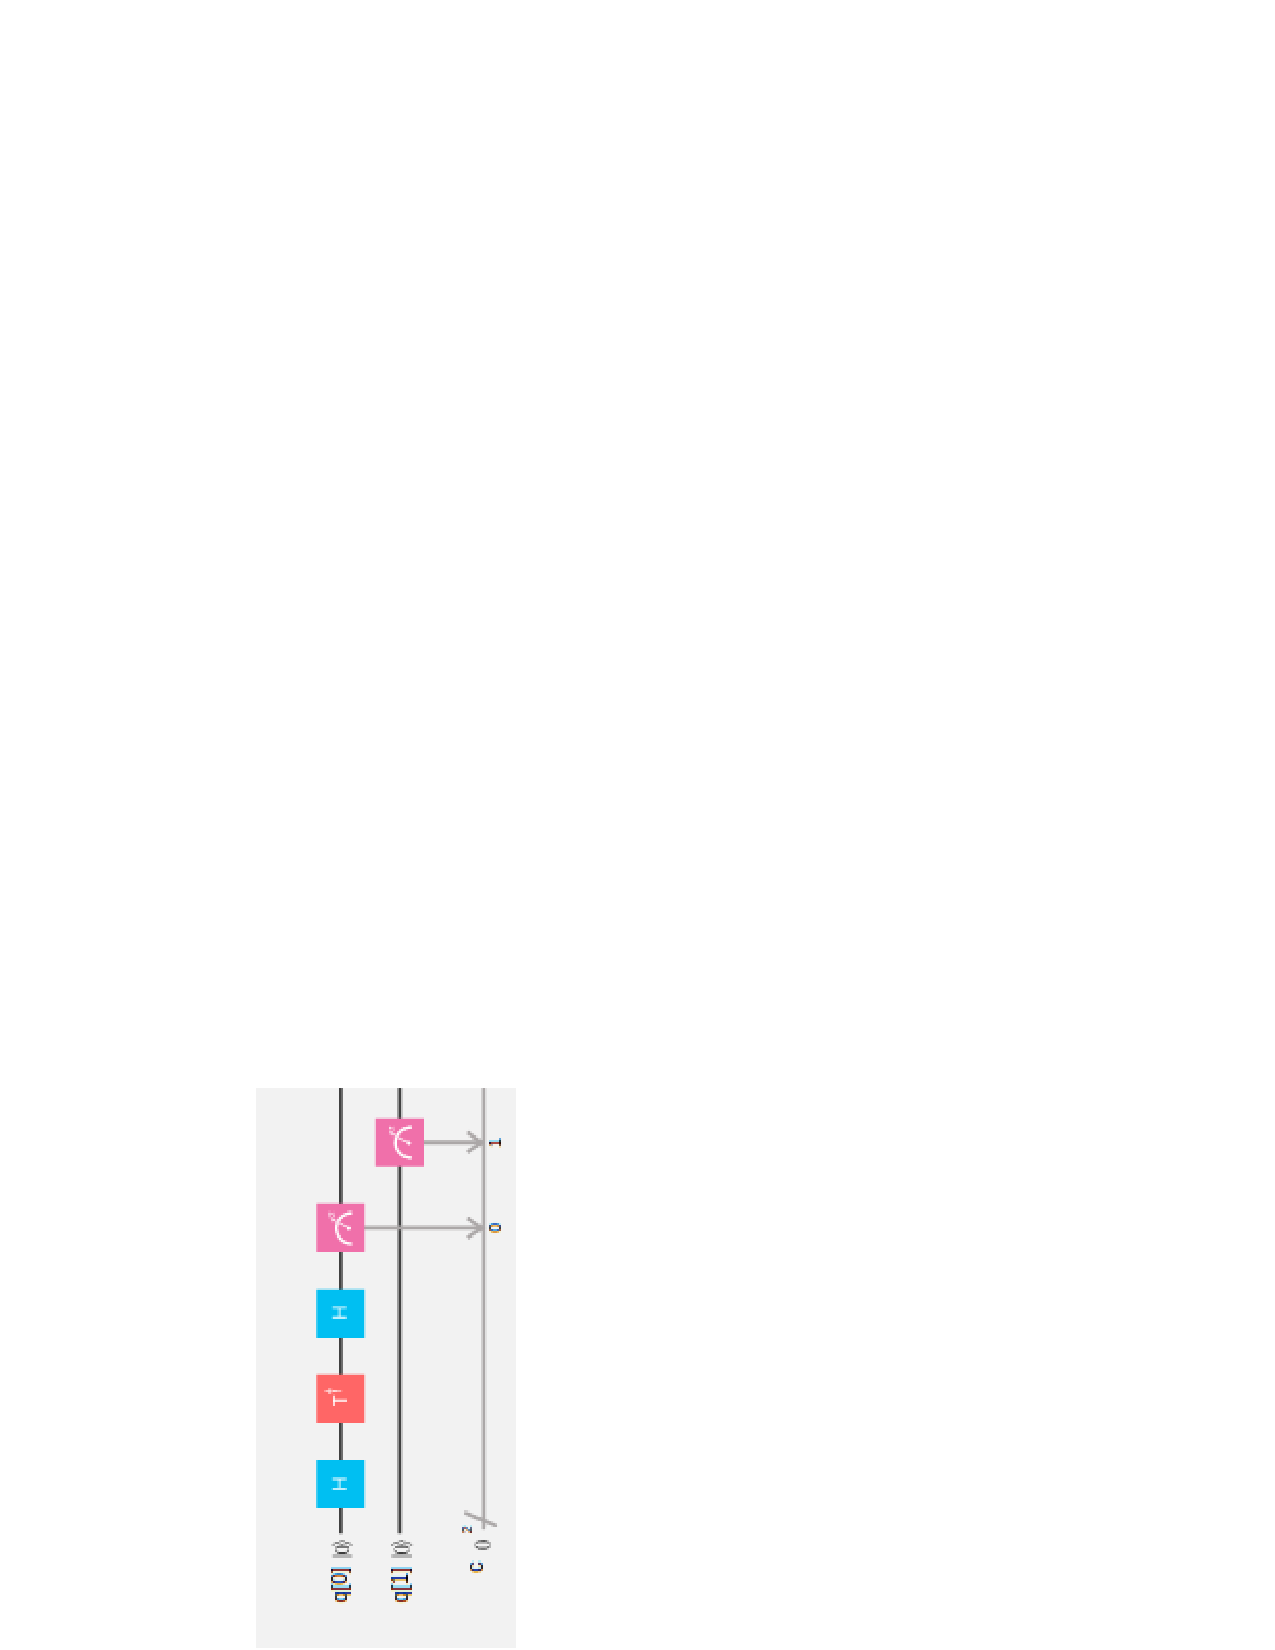
\includegraphics{future/QC-FormConstant.pdf}}}
\caption{QC Program as Quantum Experience Score}
\label{fig:future:QC Program as Quantum Experience Score}
\end{figure}

측정은 qubit z-좌표에 기반해서 1 이나 0 으로 붕괴되도록 만듭니다.
0 으로 붕괴할 확률은 다음과 같습니다:
\iffalse

Measurement causes the qubit to collapse to either one or zero, based
on the z-coordinate of the qubit.
The probability of collapse to zero is:
\fi

\begin{equation}
	\frac{1+z}{2}
\end{equation}

비슷하게, 1 로 붕괴할 확률은 다음과 같습니다:
\iffalse

Similarly, the probability of collapse to one is:
\fi

\begin{equation}
	\frac{1-z}{2}
\end{equation}

따라서, qubit 을 생각하는 한가지 (제한된) 방법은 qubit 을 붕괴 가능성에 기반해
0 과 1 을 포함한 그 사이 값의 소수라고 생각하는 겁니다.
상숟르은 $\ket{0}$ qubit 으로 시작해서 \qop{H}, \qop{S}, 그리고 \qop{T}
오퍼레이션들을 적용하는 것으로 만들어질 수 있습니다.
예를 들어, 상수 $0.14$ 는 \qop{H}, \qop{T}$^\dagger$, 그리고 또다른 \qop{H} 를
$\ket{0}$ qubit 에
Figure~\ref{fig:future:QC Program as Quantum Experience Score} 에 보인 것처럼
적용함으로써 작은 immediate 필드를 갖는 classic 컴퓨터들에서 상수를 만들때와
완전 다르지는 않은 방식으로 만들어질 수 있습니다.
하지만, IBM Q quantum 오퍼레이션들은 50-60~나노세컨드 정도를 소모하므로, 이
오퍼레이션들은 대략 150-180~나노세컨드 정도를 소모할겁니다.
두자리 숫자의 결과를 측정하는데에는 오퍼레이션들이 100 회 정도 반복될 것을
필요로 해서 준비하고 측정하는 시간을 무시하더라도 15-18 마이크로세컨드 정도를
소모할 겁니다.
그만큼의 시간동안, classic-computing floating-point 연산은 10자리 숫자의
정확도로 작은 행렬을 뒤집을 수도 있습니다.

만약 이게 QC 가 제공하는 전부였다면, QC 는 느리고 매우 저품질을 갖는 아날로그
컴퓨터가 되었을 겁니다.
디지털 컴퓨터들은 몇십년 전에 아날로그 컴퓨터를 구식으로 만들었다는 것을 놓고
볼 때, 이 비유는 많은 개발자들이 QC 를 무시하고 그대신 classic-computing
floating point 를 사용하도록 이끌 수 있을 겁니다.
하지만, QC 는 다음 섹션에서 다룰 강력한 기능들을 제공합니다.
\iffalse

Thus, one (limited) way to think of a qubit is as a fixed-point number
ranging between zero and one, inclusive, based on these probabilities
of collapse.
Constants may be formed by starting with (say) a $\ket{0}$ qubit and
applying sequences of \qop{H}, \qop{S}, and \qop{T} operations.
For example, the constant $0.14$ can be formed by applying an
\qop{H}, \qop{T}$^\dagger$, and another \qop{H}
operation on a $\ket{0}$ qubit as shown in
Figure~\ref{fig:future:QC Program as Quantum Experience Score},
in a manner not entirely unlike constant formation on classic
computers with small immediate fields.
However, given that IBM Q quantum operations consume on the
order of 50-60~nanoseconds, this series of operations would
consume around 150-180~nanoseconds.
To measure the result to two digits would require the operation to
be repeated on the order of 100 times, consuming 15-18~microseconds,
ignoring setup and measurement time.
During that time, classic-computing floating-point arithmetic could not
only invert a modest matrix, it could also do so with more than
ten digits of precision.

If this was all that QC provided, QC would be a rather slow and very
low-quality analog computer.
Given that digital computers obsoleted analog computers some decades back,
this analogy might lead many developers to ignore QC and to
use classic-computing floating point instead.
However, QC provides a powerful capability covered in the next section.
\fi

\paragraph{Entanglement}

QC 는 한쌍의 qubit 들을 \emph{entangle} 시키는 \qop{CNOT} 또는
\emph{controlled-NOT} 오퍼레이터를 갖습니다.
\qop{CNOT} 의 다른 사용은 두개의 qubit 들을 Bloch-sphere vector 에 의해 정의된
같은 값, 다른 값, 또는 (대충 말해서) 특정 값들의 조합을 갖도록 만들 수
있습니다.
Entanglement 는 잠재적으로 QC 가 커다란 최적화 문제를 매우 효과적으로 처리할 수
있게 할 수도 있는, entangle 된 변수들 사이의 관계에 제약을 구현하는데에 사용될
수 있습니다.
\iffalse

QC has the \qop{CNOT} or \emph{controlled-NOT} operator that
\emph{entangles} the pair of qubits operated on.
Different uses of \qop{CNOT} can force the two qubits to have the same
value, opposite values, or other combinations of values (roughly speaking)
defined by a Bloch-sphere vector.
Entanglement can be used to implement constraints
on the relationships of the entangled variables to each other, which
could potentially make QC handle large optimization problems very
efficiently.
\fi

여러개의 \qop{CNOT} 오퍼레이션들은 (이론상) 임의의 갯수의 qubit 들을 entangle
할 수 있는데, 이는 서로 다른 요소간의 관계를 표현하는 매우 많은
classic-computing 데이터 구조들을 이 요소들을 나타내는 qubit 들의 entanglement
로 대체할 수 있습니다.
이론 상으로, 이는 계산 복잡도를 상당히 줄일 수 있는데, Shor 의 integer
factorization 을 위한 polynomial-time
algorithm~\cite{Shor:1997:PAP:264393.264406} 이 가장 잘 알려진 예입니다.
실용적으로는, 이런 종류의 계산은 QC 하드웨어에 상당한 개선이 있길 필요로
합니다만, 그런 개선에 대한 기대를 할 이유가
있습니다~\cite{RobertMcConnell2015QC-Entangle3000Atoms}.
많은 개발자들이 QC 프로그래밍 언어의 발전을 희망할 것인데, 예를 들어, 하나의
qubit 에서 하나 이상의 quatum operation 을 하는 언어 요소를 원할 테지만, 현재의
최고 수준의 QC 는 quantum operation 들이 소중하고 주의깊게 절약되어야 한다고
이야기 합니다.
한편, 흰머리가 성성한 우리들은 classic-computing 인스트럭션들과 메모리가
조심스럽게 절약되어야 했던 젊은날의 길었던 시간들에 대한 향수를 느낄수 있을
겁니다.
\iffalse

Multiple \qop{CNOT} operations can (in theory) entangle arbitrarily
large numbers of qubits, which could replace very large numbers of
classic-computing data structures representing relationships between
different entities with entanglement of the qubits
representing these entities.
In theory, this could greatly reduce computational complexity, with
Shor's polynomial-time algorithm for integer
factorization~\cite{Shor:1997:PAP:264393.264406}
being perhaps the best-known example.
In practice, this sort of computation will require substantial
improvements in QC hardware, though there is reason to hope
for such improvement~\cite{RobertMcConnell2015QC-Entangle3000Atoms}.
Many developers might also hope for advances in QC programming languages,
for example, language constructs that do more than a single quantum
operation on a single qubit, however, the current state of the
QC art dictates that quantum operations are precious and must
be carefully conserved.
On the other hand, those of us with ample grey hair might actually
feel a tinge of nostalgia for those long-lost years of our youth when
classic-computing instructions and memory had to be just as carefully
conserved.
\fi

\paragraph{QC as Computational Accelerator}

Given the small number of qubits and limited types of operations available
on those qubits, current QC hardware is clearly not going to run anything
resembling a modern operating system, let alone a modern software stack.
Instead, QC hardware would more likely be deployed as an accelerator,
similar to a GPGPU or FPGA,
interesting speculation about quantum operating systems
notwithstanding~\cite{HenryCorriganGibbs2017QCOS}.
This situation is similar to the now-ancient external interrupt
controllers, floating-point accelerators, and vector units that have
long since been pulled onto the CPU chip.
In contrast, as we will see in Section~\ref{sec:future:Thermodynamics}, 
it is very unlikely that QC hardware will be pulled into conventional
CPUs, at least not unless future QC hardware runs at much higher
temperatures.

In the near term, there are likely to be strict precision limitations
on many types of QC computations.
For many problems this is OK.
After all if the input data is only precise to two digits, it should
be OK for the output data to be precise to only two digits.
If additional precision is required, the QC system can do the
initial computation to two digits, and this result can be used
as the starting point for a classic computation.
This has proven a useful tactic for problems whose classic-computing
algorithms converge very slowly far from the solution, but very
quickly near the solution~\cite{JakubKurzak2007MixedPrecision}.
QC would be used to handle the portion of the computation for which
classic computing is too slow, and classic computing would be used
for the portion of the computation for which QC is too inaccurate.

It is hoped that splitting the problem over classic computing and
QC hardware will result in great speedups, but there can be no denying
that it greatly complicates the programming model.

Perhaps some time in the future it will be possible to extract
state, including superposition and entanglement, from a QC system,
and then reload it at a later time.
Until this is possible, QC systems are dedicated accelerators
that cannot be context-switched, except perhaps by partitioning
a large QC system into smaller pieces, each piece being used by
a different application.
Of course, these sorts of dedicated-hardware approaches are perfectly
acceptable in situations for which a batch (rather than timesliced)
computing model is suitable.

Developers wishing more information on QC should refer to QC textbooks
and IBM's Quantum Experience~\cite{IBM2016QuantumExperience}.
Additional comparisons between QC and classic computing may be
found in Sections~\ref{sec:future:Heuristics} and~\ref{sec:future:Outlook}.

\subsubsection{Error Rate}
\label{sec:future:Error Rate}

Quantum effects are subtle and subject to errors, as has been
well-known all the way back to
Heisenberg's uncertainty priniciple~\cite{WeinerHeisenberg1927Uncertain}
(or less well-known, but even more mind-bendingly,
Bell's theorem~\cite{JohnSBell1964EPRparadox}).
Error-correcting codes have therefore been
proposed~\cite{ADCorcoles2015QuantumErrorDetection}.
Other researchers are instead working to reduce QC error
rates~\cite{PhysRevB.77.180502,PhysRevLett.107.240501,PhysRevLett.111.080502,PhysRevB.86.100506,KristanTemme2016QC-error-mitigation}.
This work has resulted in decoherence times approaching 100~microseconds,
and decoherence times are increasing dramatically, as discussed in
Section~\ref{sec:future:Quantum Computing Progress}.
However, although a 100-microseconds decoherence time is impressive for
a QC system, it does not look at all good compared to the 64-millisecond
refresh times normally specified for DRAM.\footnote{
	And these refresh times are set conservatively.
	DRAMs can typically hold charge for 1-10~\emph{seconds}.}

Furthermore, given that IBM~Q quantum operations consume on the order of
50-60~nanoseconds, it is not possible to carry out very many
operations on a given qubit before it decoheres.
For example, an algorithm requiring 10,000 quantum operations on
a single qubit must wait for order-of-magnitude advances in
the QC state of the art.

This situation should motivate additional research into extending
coherence times, and in fact a 2013 paper demonstrated coherence
times of more than
39~\emph{minutes}~\cite{KamyarSaeedi2018QC-39-minutes}.
Unfortunately, the quantum states used by this work involve atomic nuclei,
which in turn require bulky nuclear magnetic resonance (NMR) machinery
to read and write state, and the reading and the writing takes place
at 4\,K, that is, at the temperature of liquid helium.
However, between reading and writing, the temperature of the sample may
be raised to room temperature for extended periods without affecting
the quantum state.

If the NMR requirement was not bad enough, many quantum algorithms require
entanglement~\cite{PeterWSchor2001QuantumAlgorithms}.
Unfortunately, NMR systems use strong magnetic fields to align
nuclear spins, and we cannot expect the exceedingly weak magnetic
field of one nucleus to interact strongly with an adjacent nucleus,
especially not with the electron clouds in the way.\footnote{
	The magnetic fields of nuclei \emph{can} interact directly
	via the nuclear Overhauser effect~\cite{PhysRev.92.411},
	but this effect follows not merely the inverse square law,
	but instead an inverse sixth power law!}
Now, it is possible to use higher-energy nuclear state transition,
whose photons are easily able to penetrate electron clouds.
Unfortunately, these photons are also called ``gamma rays'', which enjoy
the same sterling safety reputation enjoyed by the mercury-filled steel
tubes that served as CSIRAC's mercury-delay-line memory.
Worse yet, these gamma rays must be emitted in directions precisely
aligning with the crystal lattice of whatever material is subjected
to this punishment.
On the plus side, given some magical (and radiation-proof) way to absorb
momentum at opposite faces of this crystal, one might use these highly
directional gamma rays to construct the gamma-ray laser that appears in
so many science-fiction stories.
A gamma-ray laser is no doubt an spectacularly bad idea, but there is no
denying that it is also an spectacularly cool bad idea.\footnote{
	Hey, what would happen if someone took a sample of
	cobalt-60 and used an NMR to perfectly align all of its
	atomic nuclei!~\cite{1957PhRv..105.1413W}}

Make no mistake, this 39-minute coherence time is an impressive
achievement, but in the absence
of nanoscale NMR systems~\cite{HJMamin2013QC-nanoscale-NMR} and
highly directional and highly controlled gamma rays, it is
hard to imagine creating an efficient computer based on this approach.

The extreme impracticality notwithstanding, the relatively warm operating
temperatures are important, as discussed in
Section~\ref{sec:future:Thermodynamics}.

As long as use of nuclear quantum states for QC resides in the
realm of science fiction, we must use more fragile qubits
and error correction.
One approach is use of multiple physical qubits to represent
a single logical qubit, continuously refreshing state in an
manner reminiscent of DRAM~\cite{DanielThomasSankPhD}.
The more qubits, the lower the error rate must be, with error
rates on the order of $10^{-8}$ required for algorithms using
a few hundred qubits~\cite{DanielThomasSankPhD}.

\subsubsection{Thermodynamics}
\label{sec:future:Thermodynamics}

QC computation is thermodynamically reversible, generating
very little waste heat~\cite{Bennett:1973:LRC:1664562.1664568,RichardFeynman1986QuantumMechanicalComputers}.
This means that in theory, quantum computers can avoid the
Landauer limit~\cite{Landauer:1961:IHG:1661184.1661186}
of $kT \ln 2$, where $k$ is the Boltzmann constant and $T$ is the
temperature in degrees Kelvin.
Given that the Boltzmann constant is $1.38 \times 10^{-23}$\,J/K,
and given the 0.015\,K operating temperatures that IBM's Quantum Experience
hardware runs at, this limit is indeed low: $1.43 \times 10^{-25}$\,J.

However, because of its thermodynamic reversibiltiy,
QC is governed by an even lower limit:

\begin{equation}
	\Delta E \geq \frac{\hbar}{2 \Delta t}
\end{equation}

Here $\Delta E$ is the energy required to change the qubit in Joules,
$\Delta t$ is the time taken to change the qubit in seconds, and
$\hbar$ is Planck's constant, which is $6.62 \times 10^{-34}$\,J$\cdot$s.
For the 50-nanosecond switching times of IBM's Quantum Experience
hardware, this limit is $5.52 \times 10^{-27}$\,J, more than an order
of magnitude less than the Landauer limit.

Both of these limits are incredibly small, which holds out the promise
of insanely energy-efficient computation, except that
in practice, things don't work quite so nicely.
For example, additional waste heat will be generated
by initialization and measurement of the quantum state;
by ionizing radiation;
by thermal conduction, convection, and radiation from
the QC's room-temperature surroundings;
and
by the need for quantum error correction, whether that error correction
is implemented by duplicate qubits or by duplicate runs of the QC
program.
Unfortunately, it is not just the amount of heat generated that is
important, but also the temperature at which this heat is generated.

The thermodynamic theoretical limit on the ability of a refrigerator
to transport heat from a low temperature ($T_L$) to a high temperature
($T_H$) is given by the coefficient of performance ($C_P$):

\begin{equation}
	C_P = \frac{T_L}{T_H - T_L}
\end{equation}

\begin{table}
\centering\footnotesize
\begin{tabular}{p{1.7in}|p{0.95in}}
Law of Thermodynamics
	& English Translation \\
\hline
\hline
Energy is conserved.
	& Can't win! \\
\hline
Entropy increases in closed systems.
	& Can't break even! \\
\hline
Entropy approaches a constant value as temperature approaches absolute zero.
	& Can't leave the game! \\
\end{tabular}
\caption{The Three Laws of Thermodynamics}
\label{tab:future:The Three Laws of Thermodynamics}
\end{table}

This equation is related to the ever-inconvenient Laws of Thermodynamics,
fancifully illustrated in
Table~\ref{tab:future:The Three Laws of Thermodynamics}.

The nominal temperature for IBM~Q is 15~millikelvins, which certainly
qualifies as a low $T_L$.
Let's assume $T_H$ is 293\,K (room temperature),
in which case $C_P$ is $0.000051$.
This in turn means that it requires \emph{at least} one watt of
power into the refrigeration unit to transport $0.000051$~watts
of waste heat from the 15~millikelvin IBM~Q out to room temperature.
Put another way, 19.5\,kW is required to remove one watt of waste heat.
Thus, ``very little waste heat'' can nevertheless generate a significant
power bill for refrigeration, albeit less than two-thirds of the power
consumption of the CSIRAC machine discussed in
Section~\ref{sec:future:Quantum Computing Challenges}.
In addition, efficiently transporting data across such a large
temperature differential can be challenging.
These are but two reasons why you should not expect an IBM~Q in your
smartphone just yet.
This situtation will also prevent current QC hardware from being pulled
onto the CPU chip---the refrigeration costs would be prohibitive for
a full-power chip, even allowing for the lower-power circuitry possible
at low temperatures.\footnote{
	Interestingly enough, ARM's low-power CPU family would face
	a less daunting refrigeration barrier to QC-on-a-chip.}

\begin{table}
\centering\footnotesize
\begin{tabular}{l|r|r|r}
	&	&	& Power per watt \\
Situation
	& $T$ (K)
		& $C_P$	& waste heat (W) \\
\hline
\hline
Dry Ice
	& $195$
		& $1.990$
			& 0.5 \\
\hline
Liquid N$_2$
	& $77$
		& $0.356$
			& 2.8 \\
\hline
Liquid H$_2$
	& $20$
		& $0.073$
			& 13.7 \\
\hline
Liquid He
	& $4$
		& $0.0138$
			& 72.3 \\
\hline
IBM~Q	& $0.015$
		& $0.000051$
			& 19,500.0 \\
\end{tabular}
\caption{Refrigeration Power Consumption}
\label{tab:future:Refrigeration Power Consumption}
\end{table}

One way to reduce the barrier to QC-on-a-chip would be to raise
QC's operating temperature.
Higher temperatures help because the refrigeration power required
decreases dramatically with increasing temperature, as shown in
Table~\ref{tab:future:Refrigeration Power Consumption}.
Therefore, high-temperature quantum systems amenable for QC use would
greatly improve energy efficiency and ease transfer of data to and from
the QC.
Unfortunately, given the current state of the QC art, higher
temperatures also sharply decrease coherence times.
Therefore, for the foreseeable future, QC systems will need
energy-hungry refrigeration systems, which means that QC
systems need a high-value killer app.

Of course, if the value of the killer app is sufficiently high,
19.5\,kW might be considered cheap.
In this case, in the spirit of
``plenty of room at the bottom''~\cite{RichardPFeynman1959RoomAtBottom},
we might want even lower temperatures.
For example, Bose-Einstein condensates
(BECs)~\cite{NIST2001BoseEinsteinCondensate}
form in the sub-microkelvin range, exhibiting interesting
macro-scale quantum effects.
It is not clear how one would construct any sort of computer from
these condensates, nor how one would go about providing the 1.6\,GW
required to remove one watt of waste heat from a BEC---after all,
even Emmett Brown's fictional flux capacitor required only 1.21 gigawatts.
However, much remains to be explored in this realm
of low-temperature exotic states of matter and energy, to say
nothing of new materials, for but one example,
perovskite~\cite{ZhengChen2016PerovskiteQDMOFthinFilm}.
Other avenues include increased pressure, given that diamond anvil
cells~\cite{Weir1959DiamondAnvilCell} can now reach
640\,GPa~\cite{LeonidDubrovinsky2012640GPaDiamondAnvilCell},
which is almost double the estimated pressure at the center of the earth.
Such exploration is of course pure research, but if QC is at 1940s levels
of development, pure research should have a significant role to play.

Either way, a killer app is absolutely necessary.
Optimization might well be one such killer app, but as we will see in the
next section, it has serious competition.

\subsubsection{Heuristics}
\label{sec:future:Heuristics}

Moore's Law for SAT~\cite[Fig.~2.3]{Kroening:2008:DPA:1391237} shows
that industrial-strength SAT solvers have advanced from handling
``in a few hours'' about
100 variables in 1990 to handling about 1,000,000 in 2010, an increase
of four orders of magnitude in 20 years.
This represents a doubling every 1.5 years, and this progress has
continued.
For example, in 2016, a software-verification application solved a
90,000,000-variable problem in 84 hours~\cite{LihaoLiang2016VerifyTreeRCU}.
Others have noted similar exponential
progress~\cite{SharadMalik2010SATSolverHistory,SATCompetition2002,vanHarmelen:2007:HKR:1557461,Malik:2009:BST:1536616.1536637,JamesEzick2014ExtremeSAT}.
This progress has been due to great advances in SAT-solver
heuristics~\cite{Kroening:2008:DPA:1391237,Zhang:2002:QEB:647771.734434,SharadMalik2010SATSolverHistory,Malik:2009:BST:1536616.1536637,Audemard:2009:PLC:1661445.1661509}.

Although there are special SAT cases that have not yet succumbed to
heuristics, perhaps most famously those requiring application of the
pigeonhole principle~\cite[page~38]{Kroening:2008:DPA:1391237},
it seems safe to assume continued progress.
And similar progress has also been achieved for other hard
problems~\cite{WikipediaPrimalityTest,WikipediaTSP,WikipediaIntegerFactorization}.
This should not be surprising, given that there is great economic value
in improving logistics, hardware/software verification, electronic layout,
and other problems that reduce to SAT or to other famous hard problems.
This value can be expected to continue to drive significant research
and development in this area, perhaps incorporating additional
machine-learning work~\cite{ShaiHaim2009SAT-MachineLearning}.
For example, perhaps machine-learning techniques will allow difficult
cases to be detected so that alternative solution methods can be applied
as needed.

Of course, much of this work has been heuristic and/or probabalistic,
so it might at first glance seem unfair to compare them to
QC algorithms.
However, QC algorithms are inherently probabilistic due to error rates
and measurement uncertainties, so the comparison is in fact eminently
fair.
This could be a severe challenge to mainstream QC, given the potential
need for 90,000,000 qubits to address problems recently solved by
very ordinary classical single-threaded SAT
solvers~\cite{LihaoLiang2016VerifyTreeRCU}.

Nor are these considerations solely theoretical.
There has been work documenting a four-orders-of-magnitude
performance advantage of D-Wave machines compared to classical
software for certain algorithms~\cite{McGeoch:2013:EEA:2482767.2482797}.
This work achieved considerable traction in the popular
press~\cite{CharlesChoi2013D-WaveGoogleNASA}.
However, another researcher has shown that classical software running
single-threaded on desktop-class systems can
have four-order-of-magnitude performance advantages over
D-Wave hardware~\cite{AlexSelby2014D-Wave-vs-classical,AlexSelby2013D-WaveHarderQUBO}.
Still other researchers found no evidence of quantum speedup
from D-Wave hardware for selected problems, though there might well be
other problems for which D-Wave hardware produces such
speedups~\cite{AdrianCho2014QC-D-WaveNoSpeedup,TroelsFRonnow2014QC-D-WaveNoSpeedup}.
Perhaps surprisingly, a D-Wave researcher argues that the search for
quantum speedup is in some sense
problematic~\cite{MohammadHAmin2015QC-D-Wave-QuantumSpeedupProblematic},
however, it really does appear that evaluating QC system performance is
not at all
trivial~\cite{PhysRevLett.118.100601,ArsTechnica2017QC-SpeedTradeoffs}.

Nevertheless, limitations in hard-problem heuristics such as the
pigeonhole principle for SAT
solvers~\cite[page~38]{Kroening:2008:DPA:1391237}
provides some hope that a high-value QC killer app might someday emerge.

Unfortunately, heuristics are not the only threat to the utility
of QC systems.
Advances in mathematics might also be a potent threat, as we will see
in the next section.

\subsubsection{Mathematical Advances}
\label{sec:future:Mathematical Advances}

One of the more tantalizing promises of QC is Shor's
polynomial-time integer factorization
algorithm~\cite{Shor:1997:PAP:264393.264406,WikipediaShorsAlgorithm}.
However, current polynomial-factoring algorithms are not
inconsequential.
For example, the \co{maxima} program can factor a 59-digit number\footnote{
	\scriptsize
	63698321299468802831035558537099113360211126822411635339497,
	which is the product of 15780285428767, 15780285428771, and
	255798667878176814448339699861021.}
in less than 20 seconds single-threaded on an x86 laptop.
Of course, this is a very small number compared to the 1,000-digit
integers that would need to be factored in order to break RSA,
and if integer factorization is exponential, RSA is quite safe.

However, an unexpected classic-computer
polynomial-time integer primality test was recently
devised~\cite{ManindraAgrawal2004PrimesIsInP,WikipediaAKSPrimalityTest}.
Who is to say that a classic-computer polynomial-time integer
factorization algorithm won't soon follow?

It is all too easy to dismiss the possibility of mathematical solutions
to hard problems.
One way to avoid succumbing to this temptation is to consider the
long list of major advances over the last 50 years:

\begin{description}
\item[1970:] Proof that Hilbert's 10\textsuperscript{th} problem
	is unsolvable.
\item[1975:] Fractals.
\item[1976:] Proof of the four-color problem.
\item[1984:] First polynomial-time algorithm for solving linear
	programming problems.
\item[1994:] Proof of Fermat's Last Theorem.
\item[1998:] Proof of Kepler's conjecture.
\item[2002:] Polynomial-time integer primality test.
\item[2002:] Proof of Catalan's conjecture.
\item[2003:] Proof of the Poincar\'e conjecture.
\item[2004:] Proof of the classification of finite simple groups.
\item[2013:] Proof that there is no bound on the values of
	pairs of primes differing by a finite number.
\item[2015:] Quasi-polynomial time solution to the graph isomorphism
	problem.
\end{description}

Several of these problems had stood for centuries, perhaps most famously
Fermat's Last Theorem.
The 2013 prime-pair result represents the first significant step forward
on Euclid's 300BC twin-prime hypothesis, that is to say, the first
significant step forward in more than two millennia.

Perhaps there is a race to solve hard problems in mathematics on
the one hand and to perfect large-scale quantum computing on
the other.
If so, we can hope that the competition between these two approaches
will be good for all concerned.
The next section assesses QC's outlook based on its current
competitive position with respect to classical computing.

\subsection{Outlook}
\label{sec:future:Outlook}

So what is required for QC to take over the world?

This section looks at two aspects of this question:
(1)~``What is needed to make a production-quality QC system?'' and
(2)~``What is the QC killer app?''

\subsubsection{Production-Quality QC Systems}
\label{sec:future:Production-Quality QC Systems}

An industrial-strength QC system requires per-qubit error rates below the
$10^{-8}$ threshold, preferably far below.
Shor's algorithm requires that a great many of these qubits be entangled,
and also requires several thousand general-purpose qubits.
Beating classical SAT solvers will require many millions of qubits.
It must be possible to load data into and extract results from QC
systems with high bandwidth and low latency.
The power consumption of a QC system (including refrigeration) must be
commensurate with the value of the problem being solved, and must also
be competitive with classical computing systems solving the same problem.

At some point, an agreed-upon measure of the overall capability of a
QC system will be needed.
One early candidate is the concept of
\emph{quantum volume}~\cite{LevSBishop2017QuantumVolume}, which
incorporates number of qubits, number of operations until decoherence,
connectivity, and parallelism.
Past experience with other technologies indicates that quite a few more
measures will be proposed, with some being more self-serving than others.
Should multiple QC killer apps appear, it is likely that specialized
measures will be tuned to the requirements of a given app.

Of course, such specialization requires that there actually be killer
apps, which leads to the next section.

\subsubsection{QC Killer Apps}
\label{sec:future:QC Killer Apps}

This section evaluates five potential QC killer apps,
Simon's periodicity problem,
Shor's integer factorization algorithm,
Grover's search algorithm,
quantum mechanical dynamics,
optimization problems, and
gaming.

\paragraph{Simon's Periodicity Problem}
\label{sec:future:Simon's Periodicity Problem}

Simon's problem, as described by
Shor~\cite{PeterWSchor2001QuantumAlgorithms},
requires computing the periodicity of a function.
Let's assume that there is no polynomial-time classical
algorithm solving this problem.
The question then becomes ``Why is solving this problem valuable?''
At present, there is no known valuable use for this algorithm.

\paragraph{Shor's Integer Factorization Algorithm}
\label{sec:future:Shor's Integer Factorization Algorithm}

Shor's algorithm factors integers in polynomial time.
This result would be quite valuable (if rather destructive),
but current QC systems are nowhere near able to run
Shor's algorithm on the thousand-digit numbers required
to break RSA cryptography.
This algorithm requires general-purpose highly entangled qubits,
so we must start with IBM~Q's May 2017 sixteen-qubit system.
Assuming D-Wave's 1.4~years per doubling, it will be about thirteen
years before QC systems can break current-day RSA.
% 1000 digits is about 1000*l(10)/l(2)=3322 bits
% Assume 1 qubit per bit for Shor's algorithm.
% At D-Wave doubling rate: 1.4*l(3322/16)/l(2)=13.1 years
On the other hand, if IBM sustains its 8-month doubling time, RSA has
less than five years to live.
% IBM from 5 to 16 qubits in a year: l(2)/l(16/5)=.59592202035757028109 years
% This is 12*l(2)/l(16/5)=7.15 months.
% So at IBM doubling rate: 0.5959*l(3322/16)/l(2)=4.6 years.
Of course, both cases assume that QC surmounts the challenges called
out in Section~\ref{sec:future:Quantum Computing Challenges}.
Furthermore, it seems likely that a real implementation of Shor's
algorithms would need additional qubits, which might significantly extend
RSA's lifespan.

Even those who are only slightly paranoid might consider it to be not
too early to start thinking in terms of replacing RSA.

\paragraph{Grover's Search Algorithm}
\label{sec:future:Grover's Search Algorithm}

Grover's algorithm searches an unordered list of N items
in $O(\sqrt N)$ time.
But before this can happen, the list must be downloaded into
the QC system.
The competing classical system can use this time to construct
any desired index over the data, after which the classical
system can carry out the search in $O(\log N)$ time, which
is much faster than the $O(\sqrt N)$ time promised by
Grover's algorithm.
Of course, this would change if the data originates in the
QC system.
However, given the large capacities and low costs of
classical mass storage, we can expect the bulk of the data to remain
in classical systems for the foreseeable future.

Some believe that Grover's algorithm might also be applied to more general
searches, including searching for solutions to optimization problems.
Optimization via QC is taken up later in this section.

\paragraph{Quantum Mechanical Dynamics}
\label{sec:future:Quantum Mechanical Dynamics}

Simulating quantum mechanical dynamics.
It is believed that QC systems will be able to simulate themselves
exponentially faster than classical systems will be able to
simulate QC systems~\cite{Feynman1982}.
However, the geometric constraints inherent in manufacturable
QC systems suggests that classical systems have a chance
to efficiently simulate quantum systems with less
manufacturing-friendly geometries.
Microsoft is nevertheless betting on quantum chemistry as being
the initial QC killer app~\cite{TomSimonite2017QC-MS-Chemistry},
perhaps based on reconfigurable QC hardware.
Nor is Microsoft alone: Chinese researchers are working to apply
QC to model quantum photon interactions~\cite{StephenChen2017ChinaQC}.
In addition, IBM calls out chemistry as a possible QC application.

In any case, given that quantum chemistry requires solving
Schr\"{o}dinger's equation, which in turn can require inverting
gigabyte-sized sparse matrices, progress in this area would
be quite valuable.
One of QC's competitors might be machine learning, given the positive
experiences with \url{https://fold.it}.
It is also possible that another competitor might turn out to be the
molecules themselves~\cite{Chin-wenChou2017ManipulateMolecule}, though
currently these methods are restricted to very small molecules.
So quantum chemistry might be QC's best killer-app bet.

\paragraph{Optimization Problems}
\label{sec:future:Optimization Problems}

Earlier sections have discussed D-Wave's target market of optimization
problems.
Assuming that a QC algorithm for solving SAT requires only one qubit
per variable, and assuming that D-Wave continues doubling qubits every
1.4 years, it will be 35 years before a D-Wave machine can reproduce
Liang's SAT-based Linux-kernel RCU correctness
proof~\cite{LihaoLiang2016VerifyTreeRCU}.

Improved solutions to the famous Traveling Salesman Problem would
be extremely valuable in reducing costs (and environmental impacts)
of logistics, but current classic heuristics can find near-optimal
solutions for hundreds of cities~\cite{Martin:1992:LMC:2307953.2308141}
and polynomial-time algorithms that are guaranteed to find routes
that are no more than 40\% longer than optimal for arbitrarily
large numbers of cities\cite{Sebo:2014:STN:2688265.2688281},
improving on the 50\% bound located a few decades
earlier~\cite{NicosChristofides1976TSP-FiftyPercent}.
As of 2006 TSP solvers were finding optimal solutions to
85,900-city problems~\cite{DLApplegate2007TSPtextbook}.
Assuming one qubit per city and assuming that D-Wave continues doubling
its systems' qubit counts every 1.4 years, it will take D-Wave more than seven
years to produce a system capable of handling this problem.
However, it seems likely that one qubit per road segment (rather than per city)
will be required, in which case far more qubits will be required,
resulting in a very long wait indeed.
Quantum computing might one day win this race, but there can be no doubt that
classic-computing heuristics are putting up an impressive fight.

\paragraph{Gaming}
\label{sec:future:Gaming}

No section on killer apps for any sort of computer system could possibly
be complete without some discussion of gaming.
And it turns out that the first QC computer games appeared in early
2017~\cite{JamesWootton2017IBMQEgame,JamesWootton2017IBMQEbattleship}.
These games are extremely primitive, but the real surprise is that
they exist at all.
That said, gaming and entertainment have been driving forces
behind a great many improvements in classical computing, so it is
only reasonable to assume that they will also have a role to play
in QC systems.

\paragraph{QC Killer App: Conclusions}
\label{sec:future:QC Killer App: Conclusions}

The two areas that seem to have the best chance of producing the killer
app that QC so badly needs are quantum mechanical dynamics (perhaps
most notably quantum chemistry) and optimization.
However, neither of these areas is the sole property of QC: Classical
computing is still very much in play.
In short, the jury is still out on QC, consistent with the
statement that ``this is the '40s''.

\subsection{QC Summary and Conclusions}
\label{sec:future:QC Summary and Conclusions}

Within the past decade, QC has made the move from pure theory to
commercially available systems along with publicly accessible hardware.
This is impressive progress, but the QC killer app has not yet been
identified.
One possible starting niche for QC contains problems that classic algorithms
have special difficulty with, for example, the SAT pigeonhole problem
or quantum chemistry.
That said, classic-computing algorithms and heuristics are improving
rapidly, which means that QC must hit a moving target.
The jury is therefore still out on the economic viability of QC systems,
but it seems likely that the competition between
QC and classic systems will benefit everyone.

Assuming that the QC community reacts well to this competition,
we can expect future QC systems to be as different from
today's prototypes as current classic systems are from the 1949 CSIRAC.
However, for the foreseeable future, QC systems are likely to be
architected as computational accelerators attached to classic computing
systems,
which means that large software constructs like operating systems will
continue to run on classic computing systems rather than on QC systems.
Current QC state-saving limitations suggest that QC hardware will be shared by
partitioning rather than by context switching, however, as is also
the case for a number of present-day devices that have large contexts.

Organizations and developers that can afford to do so should therefore
invest in both QC and classic systems.
However, those operating under tight constraints might reasonably choose
to continue focusing solely on classic computing systems, looking to
quantum effects only for quantum encryption/communication, which is
already used in practice.
